\newpage
1\section{Redes Neuronales}

\noindent Las redes neuronales artificiales, son un algoritmo basado en el funcionamiento de las propias neuronas del cerebro que reciben señales de entradas de las neuronas con las cuales están conectadas, las procesan y envían el resultado a las neuronas con las que estén conectadas. 

\noindent Una neurona artificial es mucho más simple que una neurona, López R. \cite{Roberto 2008} lo define de la siguiente manera: 
\begin{defi}
Una neurona procesa una entrada $\textbf{x}$ de acuerdo con unos pesos sinápticos $(b,\omega)$ que luego es transformada por una función de activación $g(u)$, las más habituales son la función sigmoide, una función lineal, la tangente hiperbólica o directamente la identidad. 

\noindent Una  vez definidos los elementos que forman una neurona artificial estos se utilizan de manera que se utiliza la función:
\begin{equation}
\begin{split}
f:\mathbb{R}^p &\longrightarrow \mathbb{R}\\
f(\textbf{x})&\longrightarrow f(\textbf{x};b,\omega)
\end{split}
\end{equation}
Donde 
\begin{equation}
f(\textbf{x})=g\left(b+\sum_{i=1}^p \omega_i x_i\right)
\end{equation}
El siguiente diagrama proporciona una forma sencilla de entender el funcionamiento de dicho modelo, incluyendo la analogía de las neuronas biológicas. 
\end{defi}
\begin{center}
%%Hay que pedirle a Carlos que lo edite por que yo la verdad que no se 
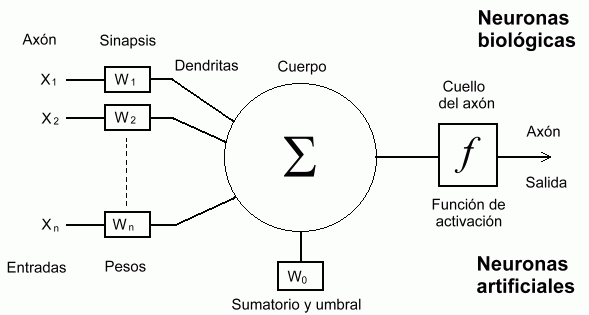
\includegraphics[scale=0.6]{Documentos Extra/Imagenes/neurona.png}
\end{center}

\noindent El potencial de este tipo de algoritmos es poder conectar neuronas unas con otras, de manera que la salida que produce una funcione de entrada para otra.
\begin{defi}
Se llama capa de neuronas a un conjunto de neuronas que tienen en común las señales de entrada y producen un vector de salidas que pueden o no servir como señal de entrada para otra. 
\end{defi}

\noindent La siguiente imagen es un esquema de una red neuronal con 7 capas de neuronas interconectadas donde la primera capa es de escalado y la última de desescalado. Se puede observar que se predicen las variables $y_1, y_2, y_3$ usando como entrada las variables $x_1,x_2,x_3,x_4$ 

\begin{figure}[h]
\centering
%%Hay que pedirle a Carlos que lo edite por que yo la verdad que no se 
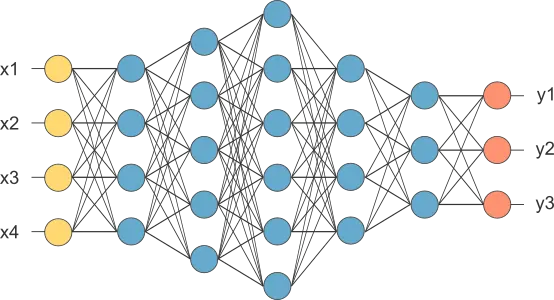
\includegraphics[scale=0.5]{Documentos Extra/Imagenes/red-neuronal-grande.png}
\caption{Imagen extraída directamente de www.neuraldesigner.com}
\end{figure}
\subsection{Proyection Pursuit Regression}

\noindent Sean un vector aleatorio \textbf{x} de longitud $p$, una variable objetivo $Y$ y una familia de vectores de parámetros de longitud $p$, $\lbrace \omega_m\rbrace_{m=1}^M$. Entonces el modelo de Regresión por Búsqueda de Proyecciones \textit{(PPR en inglés)} es de la forma :
\begin{equation}
f(\textbf{x})=\sum_{m=1}^M g_m(\omega_m^T \textbf{x})
\end{equation}

\noindent En este modelo las funciones $g_m$ no son especificadas y son estimaciones a lo largo de las direcciones de los vectores $\omega_m^T \textbf{x}$. Según \textit{Hastie, Tibshirani y Friedman} \cite{Hastie 2001} para un $M$ lo suficiente grande y utilizando las $g_m$ apropiadas este modelo puede ayudar a la predicción de cualquier función continua real. 

\noindent Para ajustar este tipo de modelos tenemos un ajuste en dos pasos, primero se estiman las funciones $g_m$ en función de los parámetros $\omega_m$ del paso anterior y luego con las $g_m$ estimadas se optimiza respecto de los parámetros $\omega_m$. Teniendo en cuenta lo siguiente :
\begin{itemize}
\item Los métodos de obtención de las $g_m$ deben producir funciones derivables. 
\item Se pueden ir actualizando tanto las $g_m$ como los $\omega_m$. Aún así, $\omega_m$ no se suele actualizar para evitar un gasto computacional excesivo. 
\item Se puede usar validación cruzada o ir comprobando si hay mejora para estimar la cantidad total de sumandos $M$.
\end{itemize}


%%Detallar

\noindent El uso de este tipo de modelos suele estar restringido así como el de las redes neuronales a la predicción, ya que suelen producir modelos de alta complejidad y difícilmente interpretables. 

\noindent Sobre este modelo se sustentan las redes neuronales, que establecen previamente las funciones de activación $g_m$.

\noindent En el caso de las redes neuronales, el método de ajuste varía al modelo previamente descrito ya que las funciones están prefijadas. 


\subsection{Red Neuronal de 2 capas }

\noindent En pos de la sencillez de los resultados, se detallará la  de una red neuronal de dos capas. El resto de casos $m\geq 2$, el proceso es análogo. Añadir que la situación es aquella en la que se quiere predecir $K$ variables objetivo a partir de observaciones de $p$ variables. 

\noindent La primera capa tiene los siguientes elementos:
\begin{itemize}
\item Como datos de entrada cada una de las observaciones $\textbf{x}$ de tamaño $p$ e incluimos en cada uno el término inicial $x_{0}=1$ de tal manera que hay $p+1$ datos de entrada.
\item Un total de $M$ unidades lo que provocará un conjunto $\lbrace z_m \rbrace$ de datos de salida.
\item Cada unidad de las $M$ tiene unos pesos $\alpha_m$ de dimensión $p+1$, donde la primera componente $\alpha_{m0}$ se denomina \textbf{sesgo}.
\item Una función de activación \textit{(Que puede o no ser lineal)} $g^{(1)}$.
\end{itemize}
\noindent De esta manera, tenemos que los datos de salida de esta primera capa son de la forma:
\begin{equation}
z_m=g^{(1)}(\alpha_m^T\textbf{x})
\end{equation}

\noindent De manera análoga tenemos una segunda capa de neuronas con los siguientes elementos:
\begin{itemize}
\item Como datos de entrada los $M$ resultados de la capa anterior, $z_m$ al que añadimos $z_0=1$ y denotaremos como el vector $\textbf{z}$ de longitud $M+1$.
\item Un total de $K$ unidades lo que provocará un conjunto $\lbrace t_k \rbrace$ de datos de salida.
\item Cada unidad de las $K$, tiene unos pesos $\beta_m$ de dimensión $M+1$ igual que en la anterior. 
\item Una función de activación \textit{(Que puede o no ser lineal)} $g^{(2)}$ que puede ser la misma que en la anterior o no.
\end{itemize}
\noindent De esta manera, tenemos que los datos de salida de esta primera capa son de la forma:
\begin{equation}
t_k=g^{(2)}(\beta_k^T\textbf{z})
\end{equation}
\noindent Hay que destacar que los datos deben estar escalados, o pueden serlo mediante una capa que los escale per sé.

\begin{defi}
Sea una matriz de datos $\textbf{X}$ de tamaño $n\times p$, resultado de observar las variables $X_1 \ldots X_p$, se llama \textit{capa de escalado} a la capa de neuronas con los siguientes elementos:
\begin{itemize}
\item Un vector de pesos con una sola componente igual a $1$ y el resto nulas. 
\item Una función de activación $g(z)=\frac{z-\mu_i}{\sigma_i}$ donde $\mu_i, \sigma_i$ son las media y desviación típica muestrales de cada variable.
\end{itemize}
\noindent El resultado de que la matriz de datos sea procesada por este tipo de capa es una matriz $\textbf{X}'$ centrada y estandarizada. 
\end{defi}

\subsection{Ajuste y uso de una Red Neuronal}

\noindent Una vez formulado el funcionamiento de una red neuronal, el ajuste de los pesos y sesgos de esta se puede plantear como un problema de minimización de la pérdida en función de los propios pesos, utilizando métodos de optimización numérica como el método del gradiente o el método de Quasi-Newton. 

\noindent Hay que tener en cuenta para seleccionar el modelo, es decir, el número de neuronas y capas, que las redes neuronales son proclives al sobreajuste. Esto es debido a la gran cantidad de parámetros que se pueden tener en una red con una complejidad media. Teniendo en cuenta esta problemática, se introduce una penalización a términos muy grandes y hace que los pesos sean parecidos a 0.

\noindent Una vez ajustados los pesos el modelo resultante puede ser complejo de interpretar, pero proporciona predicciones que potencialmente pueden ser todo lo precisas que se requieran según el número de capas y neuronas que utilicemos.  


\noindent En esta memoria se han detallado los tipos más simples de redes neuronales y de neuronas, con las cuales ya se obtiene una gran capacidad de predicción. Sin embargo, hay estructuras neuronales como las redes convolucionales o las capas LSTM cuya estructura \textit{(Llamadas así por sus siglas en inglés Long-Short Term Memory)} que permiten modelizar sistemas en que los estados futuros son afectados por los estados anteriores como pudiera ser el precio de una acción bursátil o el tiempo atmosférico.

\noindent Para evaluar el rendimiento de una red neuronal se pueden utilizar técnicas de validación cruzada o separar el conjunto de entrenamiento en entrenamiento, validación y test. 
En este proceso, se puede también hacer comparaciones entre varios modelos para elegir el número de neuronas y de capas.

\noindent Para mejorar el rendimiento de la propia red neuronal se pueden aplicar técnicas previamente a los datos como el Análisis de Componentes Principales o seleccionar las variables más significativas como se detalla en la sección de regresión que trata de ello.  
